\documentclass[tikz,border=10pt]{standalone}
\usepackage{tikz}
\usetikzlibrary{positioning, arrows.meta, fit, backgrounds, calc}

% Professional ACM/IEEE Academic Color Palette
\definecolor{acmPrimary}{RGB}{15, 60, 115}       % Deep Academic Blue
\definecolor{acmSecondary}{RGB}{35, 105, 165}   % Medium Steel Blue
\definecolor{acmAccent}{RGB}{60, 145, 205}      % Accent Blue
\definecolor{acmDarkGray}{RGB}{45, 55, 70}       % Dark Slate Text
\definecolor{acmLightBg}{RGB}{246, 248, 252}    % Box Light Background
\definecolor{acmBoxBg}{RGB}{255, 255, 255}      % Card White Fill
\definecolor{acmGroupBg}{RGB}{236, 242, 249}    % Container Fill
\definecolor{acmAnnoBg}{RGB}{240, 245, 252}     % Input/Output Box Shading

\begin{document}
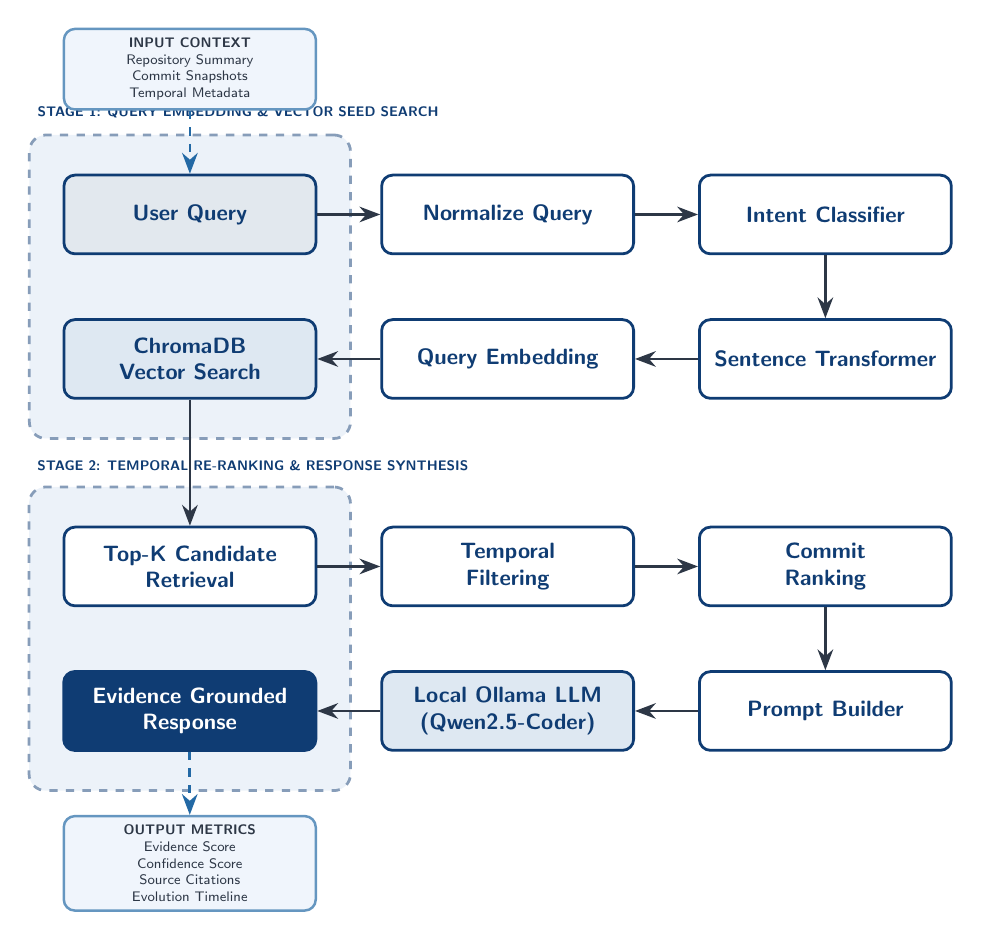
\begin{tikzpicture}[
    font=\sffamily\footnotesize,
    >=Stealth,
    node distance=0.8cm and 0.8cm,
    box/.style={
        draw=acmPrimary,
        fill=acmBoxBg,
        rectangle,
        rounded corners=4pt,
        line width=1.0pt,
        minimum width=3.2cm,
        minimum height=1.0cm,
        align=center,
        font=\sffamily\footnotesize\bfseries\color{acmPrimary}
    },
    highlight/.style={
        draw=acmPrimary,
        fill=acmPrimary,
        rectangle,
        rounded corners=4pt,
        line width=1.1pt,
        minimum width=3.2cm,
        minimum height=1.0cm,
        align=center,
        font=\sffamily\footnotesize\bfseries\color{white}
    },
    inputbox/.style={
        draw=acmSecondary!70,
        fill=acmAnnoBg,
        rectangle,
        rounded corners=4pt,
        line width=0.9pt,
        minimum width=3.2cm,
        minimum height=1.0cm,
        align=center,
        font=\sffamily\tiny\color{acmDarkGray}
    },
    header/.style={
        font=\sffamily\tiny\bfseries,
        color=acmPrimary,
        align=left
    },
    arrow/.style={
        draw=acmDarkGray,
        ->,
        line width=1.0pt
    },
    container/.style={
        draw=acmPrimary!50,
        fill=acmGroupBg,
        rectangle,
        dashed,
        rounded corners=6pt,
        line width=1.0pt,
        inner ysep=14pt,
        inner xsep=12pt
    }
]

% ================= INPUT CONTEXT =================
\node[inputbox] (input) {\textbf{INPUT CONTEXT}\\Repository Summary\\Commit Snapshots\\Temporal Metadata};

% ================= STAGE 1 =================
\node[box, fill=acmPrimary!12, below=0.8cm of input] (n1) {User Query};
\node[box, right=of n1] (n2) {Normalize Query};
\node[box, right=of n2] (n3) {Intent Classifier};

\node[box, below=0.8cm of n3] (n4) {Sentence Transformer};
\node[box, left=of n4] (n5) {Query Embedding};
\node[box, fill=acmSecondary!15, left=of n5] (n6) {ChromaDB\\Vector Search};

\draw[arrow, dashed, color=acmSecondary] (input) -- (n1);
\draw[arrow] (n1) -- (n2);
\draw[arrow] (n2) -- (n3);
\draw[arrow] (n3) -- (n4);
\draw[arrow] (n4) -- (n5);
\draw[arrow] (n5) -- (n6);

\begin{scope}[on background layer]
    \node[container, fit=(n1) (n6)] (stage1) {};
    \node[header, anchor=south west, yshift=2pt] at (stage1.north west) {STAGE 1: QUERY EMBEDDING \& VECTOR SEED SEARCH};
\end{scope}

% ================= STAGE 2 =================
\node[box, below=1.6cm of n6] (m6) {Top-K Candidate\\Retrieval};
\node[box, right=of m6] (m5) {Temporal\\Filtering};
\node[box, right=of m5] (m4) {Commit\\Ranking};

\node[box, below=0.8cm of m4] (m3) {Prompt Builder};
\node[box, fill=acmSecondary!15, left=of m3] (m2) {Local Ollama LLM\\(Qwen2.5-Coder)};
\node[highlight, left=of m2] (m1) {Evidence Grounded\\Response};

\draw[arrow] (n6) -- (m6);
\draw[arrow] (m6) -- (m5);
\draw[arrow] (m5) -- (m4);
\draw[arrow] (m4) -- (m3);
\draw[arrow] (m3) -- (m2);
\draw[arrow] (m2) -- (m1);

\begin{scope}[on background layer]
    \node[container, fit=(m1) (m6)] (stage2) {};
    \node[header, anchor=south west, yshift=2pt] at (stage2.north west) {STAGE 2: TEMPORAL RE-RANKING \& RESPONSE SYNTHESIS};
\end{scope}

% ================= OUTPUT METRICS =================
\node[inputbox, below=0.8cm of m1] (output) {\textbf{OUTPUT METRICS}\\Evidence Score\\Confidence Score\\Source Citations\\Evolution Timeline};
\draw[arrow, dashed, color=acmSecondary] (m1) -- (output);

\end{tikzpicture}
\end{document}
